\documentclass[letterpaper, 12pt]{report}

% administrivia
% (fold)
\usepackage[utf8]{inputenc}
\usepackage[T1]{fontenc}
\usepackage[english]{babel}
\usepackage[nottoc, numbib]{tocbibind}
\usepackage{hyperref}
\usepackage{pdfpages}

% alt dette for ett eksempel
\usepackage[footnotesize, bf, hang]{caption}
\usepackage{subcaption}
\usepackage{floatrow}
\usepackage{calc}
\floatsetup{ 
	heightadjust=object,
	valign=t
}

% layout
%\usepackage{fullpage}
\usepackage[sc]{mathpazo}
\usepackage{inconsolata}
\usepackage[protrusion=true,expansion=true]{microtype}
\usepackage{hyperref}
\usepackage{enumitem}
\usepackage{setspace}
%\onehalfspacing
\frenchspacing
\usepackage{listings}
\lstset{
	basicstyle=\ttfamily\footnotesize,
	tabsize=2, 
	breaklines=true
}
\usepackage{wrapfig}
\usepackage{graphicx}
% mindre tekst for sitater
\let\quoteOLD\quote
\def\quote{\quoteOLD\small}
\usepackage[bottom]{footmisc}

% citation
\usepackage[
	style=authoryear, 
	backend=bibtex, 
	dateabbrev=false
]{biblatex}
\addbibresource{references.bib}
\DefineBibliographyStrings{english}{%
	urlseen = {Retrieved},
}

% front matter
\title{\Huge \textbf{Measuring Productivity in the Software Engineering Industry}}
\author{
	Håkon S. Mork \\ 
	ORGB 423 --- Human Resources Management \\ 
	McGill University \\
	\\
	\emph{With kind contributions from Solfrid Skilbrigt of Steria}
}
\date{April 11, 2013}
% (end)

\begin{document}
\pagenumbering{roman}
\maketitle

%\cleardoublepage
\pagebreak[4] 
\thispagestyle{empty}
\null
\pagebreak[4]

% TODO update as last thing to do
\begin{abstract}
Software engineering, being mostly computer-based, lends itself well to quantitative analysis of employee productivity. 
While qualitative forms of appraisal are obviously ubiquitous, as in other fields, there are many forms of quantitative analysis that are unique to the software field.
I discuss some widely used, industry-specific quantitative and qualitative assessment techniques, and examine their strengths and weaknesses.
Managers should use quantitative measures judiciously, taking advantage of the opportunity to have an unbiased means of employee assessment while being aware of the inherent limitations. 
The company whose HR manager I interviewed uses quantitative methods only sparingly.
\end{abstract}

\tableofcontents




\chapter{Introduction}
\pagenumbering{arabic}

\section{Objectives}
As is the case for all knowledge workers, measuring the productivity of software programmers is a challenging task.
However, the software industry is more amenable to quantitative appraisal than many other forms of knowledge work, since the end result, namely software, is by its very nature easy to handle with automated processes. 

I will describe some difficulties in performing accurate, objective appraisal, as well as some approaches to quantitative evaluation that are unique to the software business.
A discussion of the pros, cons, and limitations of these methods is also provided, along with a short treatment of qualitative appraisal in the context of software development. 

Steria's use of the various appraisal techniques is discussed throughout the text. 
As the textbook's treatment of productivity measures is rather brief \parencite[][374]{textbook}, I will draw on external sources such as research and industry experts to a considerable degree.


\section{Company}
Steria is a multinational company founded in 1969 that specializes in information technology consulting, services and management. 
With headquarters in Paris and French administration, Steria is present in 16 countries and on three continents. 
The company boasts more than 20,000 employees and a 2011 annual revenue of €1.75 billion \parencite{steria:stats}.


\section{Human Resources Professional}
\begin{wrapfigure}{R}{0.3\textwidth}
	\centering
	
\includegraphics[width=\textwidth]{solfridbw}
	\caption*{Solfrid Skilbrigt}
\end{wrapfigure}
Solfrid Skilbrigt, Human Resouces Director of the Norwegian and Scandinavian branch and Deputy CEO of Scandinavia, has kindly agreed to answer my questions about human resource management in her firm. 
A graduate of the University of Trondheim, she has long and varied experience in the fields of information technology, sales, and human resources.

Her accomplishments include leading the company's employer branding, recruitment, and management and organizational development programs, as well as playing a key part in Steria's advancement to being one of the world's leading IT consulting firms. 
Skilbrigt has also been in charge of Steria's global CSR efforts since 2008.


\section{Topic Area}
Productivity in software engineering struck me as being an interesting topic because it is quite specialized and resonates well with my own background, which is in both management and computer science.
Software engineering is a comparatively young industry, having appeared in a major way only in the last few decades, and is in many respects still in its infancy.
I therefore thought it would be interesting to learn more about how one should best manage human resources in such a young and rapidly changing industry.






\chapter{Evaluation Methods and Their Limitations}

% TODO alt
\section{Challenges of Measuring Productivity}
In this section, I describe some inherent problems with quantitative assessment and accurate, objective measurement of employee productivity, with particular emphasis on challenges specific to the software engineering industry.


\subsection{Industry-Specific Problems}
Software is unlike any other kind of manmade product. 
It is intangible, complex, and most users have no idea how it works; yet they interact with it daily and spend hours upon hours staring at screens both at work and at home. 
The economics of software are also peculiar: the cost of producing large-scale software is exorbitant, but having completed it in the first place, all subsequent copies can be produced for free. 

Also unlike any other type of product, software can be made arbitrarily complex, limited primarily by how much its makers can keep in their heads at any one time. 
The complexity and intricacy of a software product tends to increase over time \parencite{veksler:truths}, and as large systems are more rarely written from scratch anymore, programmer ability to handle complexity and abstraction is key.



\subsection{Feasibility}
Whether it is possible to measure programming productivity at all is a source of some contention. For example, \textcite{fowler:cannotmeasure} echoes a common sentiment in arguing that
\begin{quote}
	Productivity, of course, is something you determine by looking at the input of an activity and its output. 
	So to measure software productivity you have to measure the output of software development---the reason we can't measure productivity is because we can't measure output. 
This doesn't mean people don't try. 
\end{quote}
The business case for objectively assessing individual performance is clear. 
It is obviously desirable for any organization to have highly productive employees, and the  difference in performance between average and exceptional employees is probably greater in the software industry than anywhere else.
Bill Gates put it succinctly:
``A great lathe operator commands several times the wage of an average lathe operator, but a great writer of software code is worth 10,000 times the price of an average software writer.'' \parencite{veksler:truths}. 

In a similar vein, \textcite{spolsky:high} analyzes empirical results that suggest that there is no correlation between effort and product quality, and concludes that the best programmers are more than an order of magnitude more productive than those at the other end of the scale. 
\textcite{martin:tenfinity} expands on the topic, stating that ``Many experts cite an order-of-magnitude productivity difference between the “best” and “average” programmers.''
It follows that an objective means of evaluating performance would be desirable. 

There are, however, may problems with such methods; \textcite[][374]{textbook} mention criteria contamination and short-term thinking as important concerns with productivity measurement in general. 
There is significant skepticism in the industry towards employing quantitative productivity assessment methods to any large degree, due to the sheer difficulty of designing good evaluation criteria. 
In a seminal article, \textcite{fenton:scientificbasis}, while presenting a somewhat more scientific set of measurement criteria than what had been common up to then, is notably pessimistic on behalf of metrics based on software complexity, asserting that ``the search for a general-purpose real-valued complexity measure is doomed to failure''. 
%Going even further, \textcite{kannan:problem} contends that it is unlikely that adequately precise measurement techniques exist; furthermore, he argues that the problem itself may be moot, and that agonizing over individual productivity should be not be the organization's main concern, as one should instead focus on customer satisfaction and keeping development schedules.

While it should be clear that quantitative tools cannot be the sole process with which to evaluate employees, and that managers should have the final say in appraisal, objective methods are a valuable addition.
%As for whether they work or not, it seems unlikely that quantitative assessment would be so widely used as it is if there were no value to organizations from it.
%Their assessments thus appear to be excessively negative, and the insufficiency of the methods we have today should not be taken as proof that it is impossible to get it right.
\textcite{angel:howto} maintains that although many within the field consider precise measurement of productivity to be difficult, there are still many genuinely useful ways to approach the problem:

\begin{quote}
	First, just because it has been done badly in the past does not mean it cannot be done well. 
	Second, as a project manager I know the capability and productivity of my staff. 
	I have to know this, otherwise I can not give good time and cost estimates. 
	I am not the only one who does this routinely. 
	Thus the measurement must be possible. 
	Third, an objective productivity measure is needed. 
	How else can one determine if any infrastructure change or any process change in worth the return on investment?
\end{quote}
One is therefore justified in staying somewhat optimistic about the usefulness and applicability of objective productivity measurement.

Nevertheless, all organizations should be aware that there are clear limitations to how much one should rely on such assessments. 
In Steria, for example, quantitative appraisal is not given precedence over qualitative results, such as appraisal from coworkers or supervisors, and is solely used as a supporting tool. 
The limitations are therefore taken into account and quantitative measurements are not given undue weight.



% \subsection{Group Effort}
% 
% The equity concerns are evident:
% If we cannot precisely compare one employee's work to that of another, is it possible to have an objective appraisal method, or are we confined to subjective assessment?





% TODO nok om specs nå?
\subsection{External Factors}
One of the perennial problems of the software industry is that neither the maker nor the clients have a precise idea of what the finished product should be like, leading to costly delays as the customer changes their mind and new requirements are added or amended even while the system is being built.
One might think that fixing this problem should be an easy matter; after all, most other engineering disciplines do not face cost overruns of the same order of magnitude that plague the software engineering trade---apart from, perhaps, the construction industry. 
This has proven not to be the case. 



As software development is an entirely abstract endeavour, often requiring considerable mental effort and concentration, quiet and appropriate working conditions are essential. 
The concept of flow \parencite{mihaly:flow} is relevant in this regard. 
Flow, also known as the ``zone'', can be summarized as a mental state of high concentration in which a person is engrossed in their work, bringing about high productivity and efficiency.
Citing the importance of flow, \textcite{spolsky:list} argues that disruption is highly damaging to programmer productivity:
\begin{quote}
If a coworker asks you a question, causing a 1 minute interruption, but this knocks you out of the zone badly enough that it takes you half an hour to get productive again, your overall productivity is in serious trouble. 
If you're in a noisy bullpen environment like the type that caffeinated dotcoms love to create, with marketing guys screaming on the phone next to programmers, your productivity will plunge as knowledge workers get interrupted time after time and never get into the zone.
\end{quote}
Steria recognizes that peace and quiet is important for productivity, and seeks to limit interruptions to as little as possible to let their employees perform to the full.
Since it is difficult to distinguish between low performance due to failure of ability, motivation, or environment when using results-based measures \parencite[][387]{textbook}, one should not rely too much on any one measure but rather compare them and look for correlations.
Trying to eliminate a bad environment as a source of low performance can therefore improve the reliability of performance appraisal in general.


One may also point out the challenge of results-based appraisal of individual employees working in teams.
Though the problem of appraising individual employees working in a team is by no means exclusive to the software engingeering business, the issue is particularly pressing in this sector.
Software engineers hardly ever work alone, and what is worse from an appraisal perspective, rarely carry out work that is easily comparable from one employee to another.
It is therefore hard for managers to draw conclusions from quantitative results-based measurements, as these are likely influenced to a significant degree by factors that have little or nothing to do with the particular employee's performance.






\section{Lines of Code}
Measuring employee productivity in terms of number of computer code lines written is a simple, widely used metric. 
However, it is also easily manipulated, often irrelevant or misleading and rarely a good indicator of individual productivity; as \textcite[][353, 374]{textbook} detail, focussing on a narrow set of criteria can be not only uninformative, but in fact damaging to the organization, since it promotes practices that may not be optimal for the organization as a whole. 
This is the case with measuring code size since it promotes verbosity, while keeping the size of the code as small as reasonably possible is usually counted as beneficial. 
Similarly, structuring code into reusable parts is widely considered to be best practice; that is, not duplicating code that is similar or identical but instead organizing it such that it may be used by many different parts of the program as needed. 
By not doing this, and instead duplicating functionality, the size of the code can be increased considerably, the cost of maintainability and clarity \parencite{veksler:truths}.

A further argument against using code line count is that code size often has no bearing on the functionality of the program \parencite{albrechtgaffey:linesofcode}. 
As an example, consider the code snippets in two different programming languages in figure \ref{fig:codelineexample}. 
Both these programs do exactly the same thing: prompt the user for a number, and then display the numbers from 1 up to that number. 
Even so, the one written in the C programming language is four times longer than the one written in the Python programming language. 
Is an employee who writes the longer one four times as productive as someone who writes the shorter one? 
Clearly not, since they both solve the same problem---but while the programmer who wrote the terser version may move on to new problems to solve, the programmer who writes more verbosely takes longer to finish the task, simply because there is more typing to be done. 
In addition, one should take into consideration the extra time spent on debugging the verbose version: 
Much like how a mechanical engineer seeks to minimize the number of moving parts in a machine, a software engineer seeks to write as little code as possible, since everything that is ``moving'' is a potential source of errors and malfunctions. 

% language length example
% (fold)
\newsavebox{\pythonexample}
\begin{lrbox}{\pythonexample}
\begin{lstlisting}
n = int(input())
for i in range(1, n + 1):
	print i
\end{lstlisting}
\end{lrbox}

\newsavebox{\cexample}
\begin{lrbox}{\cexample}
\begin{lstlisting}
#include <stdio.h>
int main(int argc, char **argv) 
{
	int n;
	scanf("%d", &n);
	int i;
	for (i = 1; i < n + 1; i++) 
	{
		printf("%d\n", i);
	}
	return 0;
}
\end{lstlisting}
\end{lrbox}

\begin{figure}
\ffigbox{
	\begin{subfloatrow}
		\ffigbox[\FBwidth+1em]{\usebox{\cexample}}{\subcaption{Example in C}}
		\ffigbox[\FBwidth+1em]{\usebox{\pythonexample}}{\subcaption{Example in Python}}
	\end{subfloatrow}
}
{\caption{These two pieces of computer code, in two different programming languages, do exactly the same thing---yet one is four times longer than the other.}\label{fig:codelineexample}}
\end{figure}
% (end)

This may be a trite observation when discussing the example in figure \ref{fig:codelineexample}, with twelve lines of code instead of three, but the principle is more general; large projects can have code line counts in the hundreds of thousands or even millions, necessitating a structured approach to development. 
Indeed, \textcite{graham:succinctness} argues that terseness is one of the programmer's prime virtues:
``[S]uccinctness is power, or is close enough that except in pathological examples you can treat them as identical.
It seems to me that succinctness is what programming languages are for.''
Thus measuring the number of lines of code an employee writes is at best irrelevant and at worst misleading. 
Still, this metric is widely used, mainly due to the ease with which one can implement an appraisal system based on it. 
Automated tools can easily count the number of code lines written by a single person in a single day, making it easy to track an employee's output over time. 
While the amount of code a single person writes is no solid indicator of their personal productivity, the amount of code that, in total, makes up a project is a decent gauge of the project's size and scope. 
\textcite{fowler:cannotmeasure} argues that

\begin{quote}
I can be pretty confident that a 100 \textsc{kloc}\footnote{Thousand lines of code.} system is bigger than a 10 \textsc{kloc} system. But if I've written the 100 \textsc{kloc} system in a year, and Joe writes the same system in 10 \textsc{kloc} during the same time, that doesn't make me more productive. Indeed, I would conclude that our productivities are about the same, but my system is much more poorly designed.
\end{quote}

On that account, code lines should be used solely as a measure of project size and complexity, not individual productivity. 
This is the way Steria uses code size: 
Only as an indicator of project size, not as an accurate measure of productivity, since it is easy to game and doing so it detrimental to the project in the long run.
This philosophy is in line with what \textcite{textbook} say on the topic of incentive conflicts:
``[a]ppraisals may inadvertently encourage employees to `look good' on a short-term basis, while ignoring the long-term ramifications'' (p. 374).
Furthermore, the textbook argues that both the results and the methods used to achieve them should be considered when one draws conclusions based on productivity measures, which is what Steria does by using not using code size as a measurement of anything else than what it is supposed to be.

% (end)




% TODO done?
% se fowler for startpunkt
\section{Function Points}
% (fold)
Counting function points is a different, but related way of measuring how much an employee has contributed to a project. 
The essential philosophy is that contributions should be measured by how much functionality they impart to the product, rather than how much typing and thinking (or other kinds effort) that went into providing that functionality. An extensive introduction is given in \textcite{symons:functionpoints}.
Function point analysis was developed by Allan Albrecht at IBM in the late 1970s, and at present, there are a number of formalized, international standards on how to measure function points, most prominently \parencite{iso:functionpoints}. 
The presence of standards strengthens the impression of function point analysis as a objective, nonbiased means of assessment.


Function points are therefore more telling than code lines in terms of benefit to the client, since providing functionality to the customer is after all the final goal of any project.
An added benefits over code line counting is that this method sideskirts the whole issue of language differences and the individual employee's style of expression, and simply focusses on the magnitude of individual contributions with respect to the finished product. 

Counting function points can be understood as ticking a metaphorical box on a checklist of desired features. 
A clear limitation is that not all features are equally important, urgent, or difficult to implement. 
This method thus requires judicious oversight to determine what parts are important and not, what tasks are difficult and not, etc.
Although requiring manual oversight to some extent defeats the purpose of having automated appraisal in the first place, some supervision and discernment is required for the function point method to give valid and reliable results. 

To be able to make accurate judgement calls, the astute manager should clearly stay informed of the product details and know in detail what their team is working on at any time.
This calls for extensive knowledge of the problem domain on the manager's part, skills that not all managers necessarily have.
\textcite{textbook} emphasize (p. 360-364) the need for appraisers to be trained in how to use the organization's appraisal process effectively and provide useful feedback to employees.

While the discussion in the textbook largely emphasizes the desire for avoiding common pitfalls such as leniency, strictness, or recency error, using a more technically involved appraisal process such as function point analysis demands technical expertise on the appraiser's part.
Hence, the manager should assess his or her own knowledge and technical faculties before making the decision on whether to use function points as an evaluating metric for their team.
The organization should make sure that supervisors have sufficient technical proficiency before implementing function point analysis, and should carry out exhaustive training and instruction if that is not the case, which may be a costly affair.
Steria considers function point analysis impractical and overly technical and does not use it.


% (end)

% TODO cyclomatic, halstead
\section{Cyclomatic Complexity}
% (fold)
Cyclomatic complexity is a mathematically precise assessment method based on a flowchart-like representation of a computer program called a control flow graph. 
This method was developed by \textcite{mccabe:cyclomatic}, and has been widely applied since \parencite{nist:cyclomatic}, mostly for testing and quality assurance purposes. 
The analysis hinges on the so-called ``cyclomatic number'' of a piece of code, which is computed as $E - N + P$, where $E$ is the number of edges, $N$ is the number of nodes, and $P$ is the number of start and end points in the associated graph. 
Figure \ref{fig:cyclomatic} has two simple examples of what a control flow graph might look like; the left one, for example has a cyclomatic number of $9-7+1=3$.
Being entirely mathematical, cyclomatic complexity is well suited to automation, and is arguably \parencite{angel:howto} a fairly accurate metric of the perceived complexity of a piece of software. 

\begin{figure}[t]
	\centering
	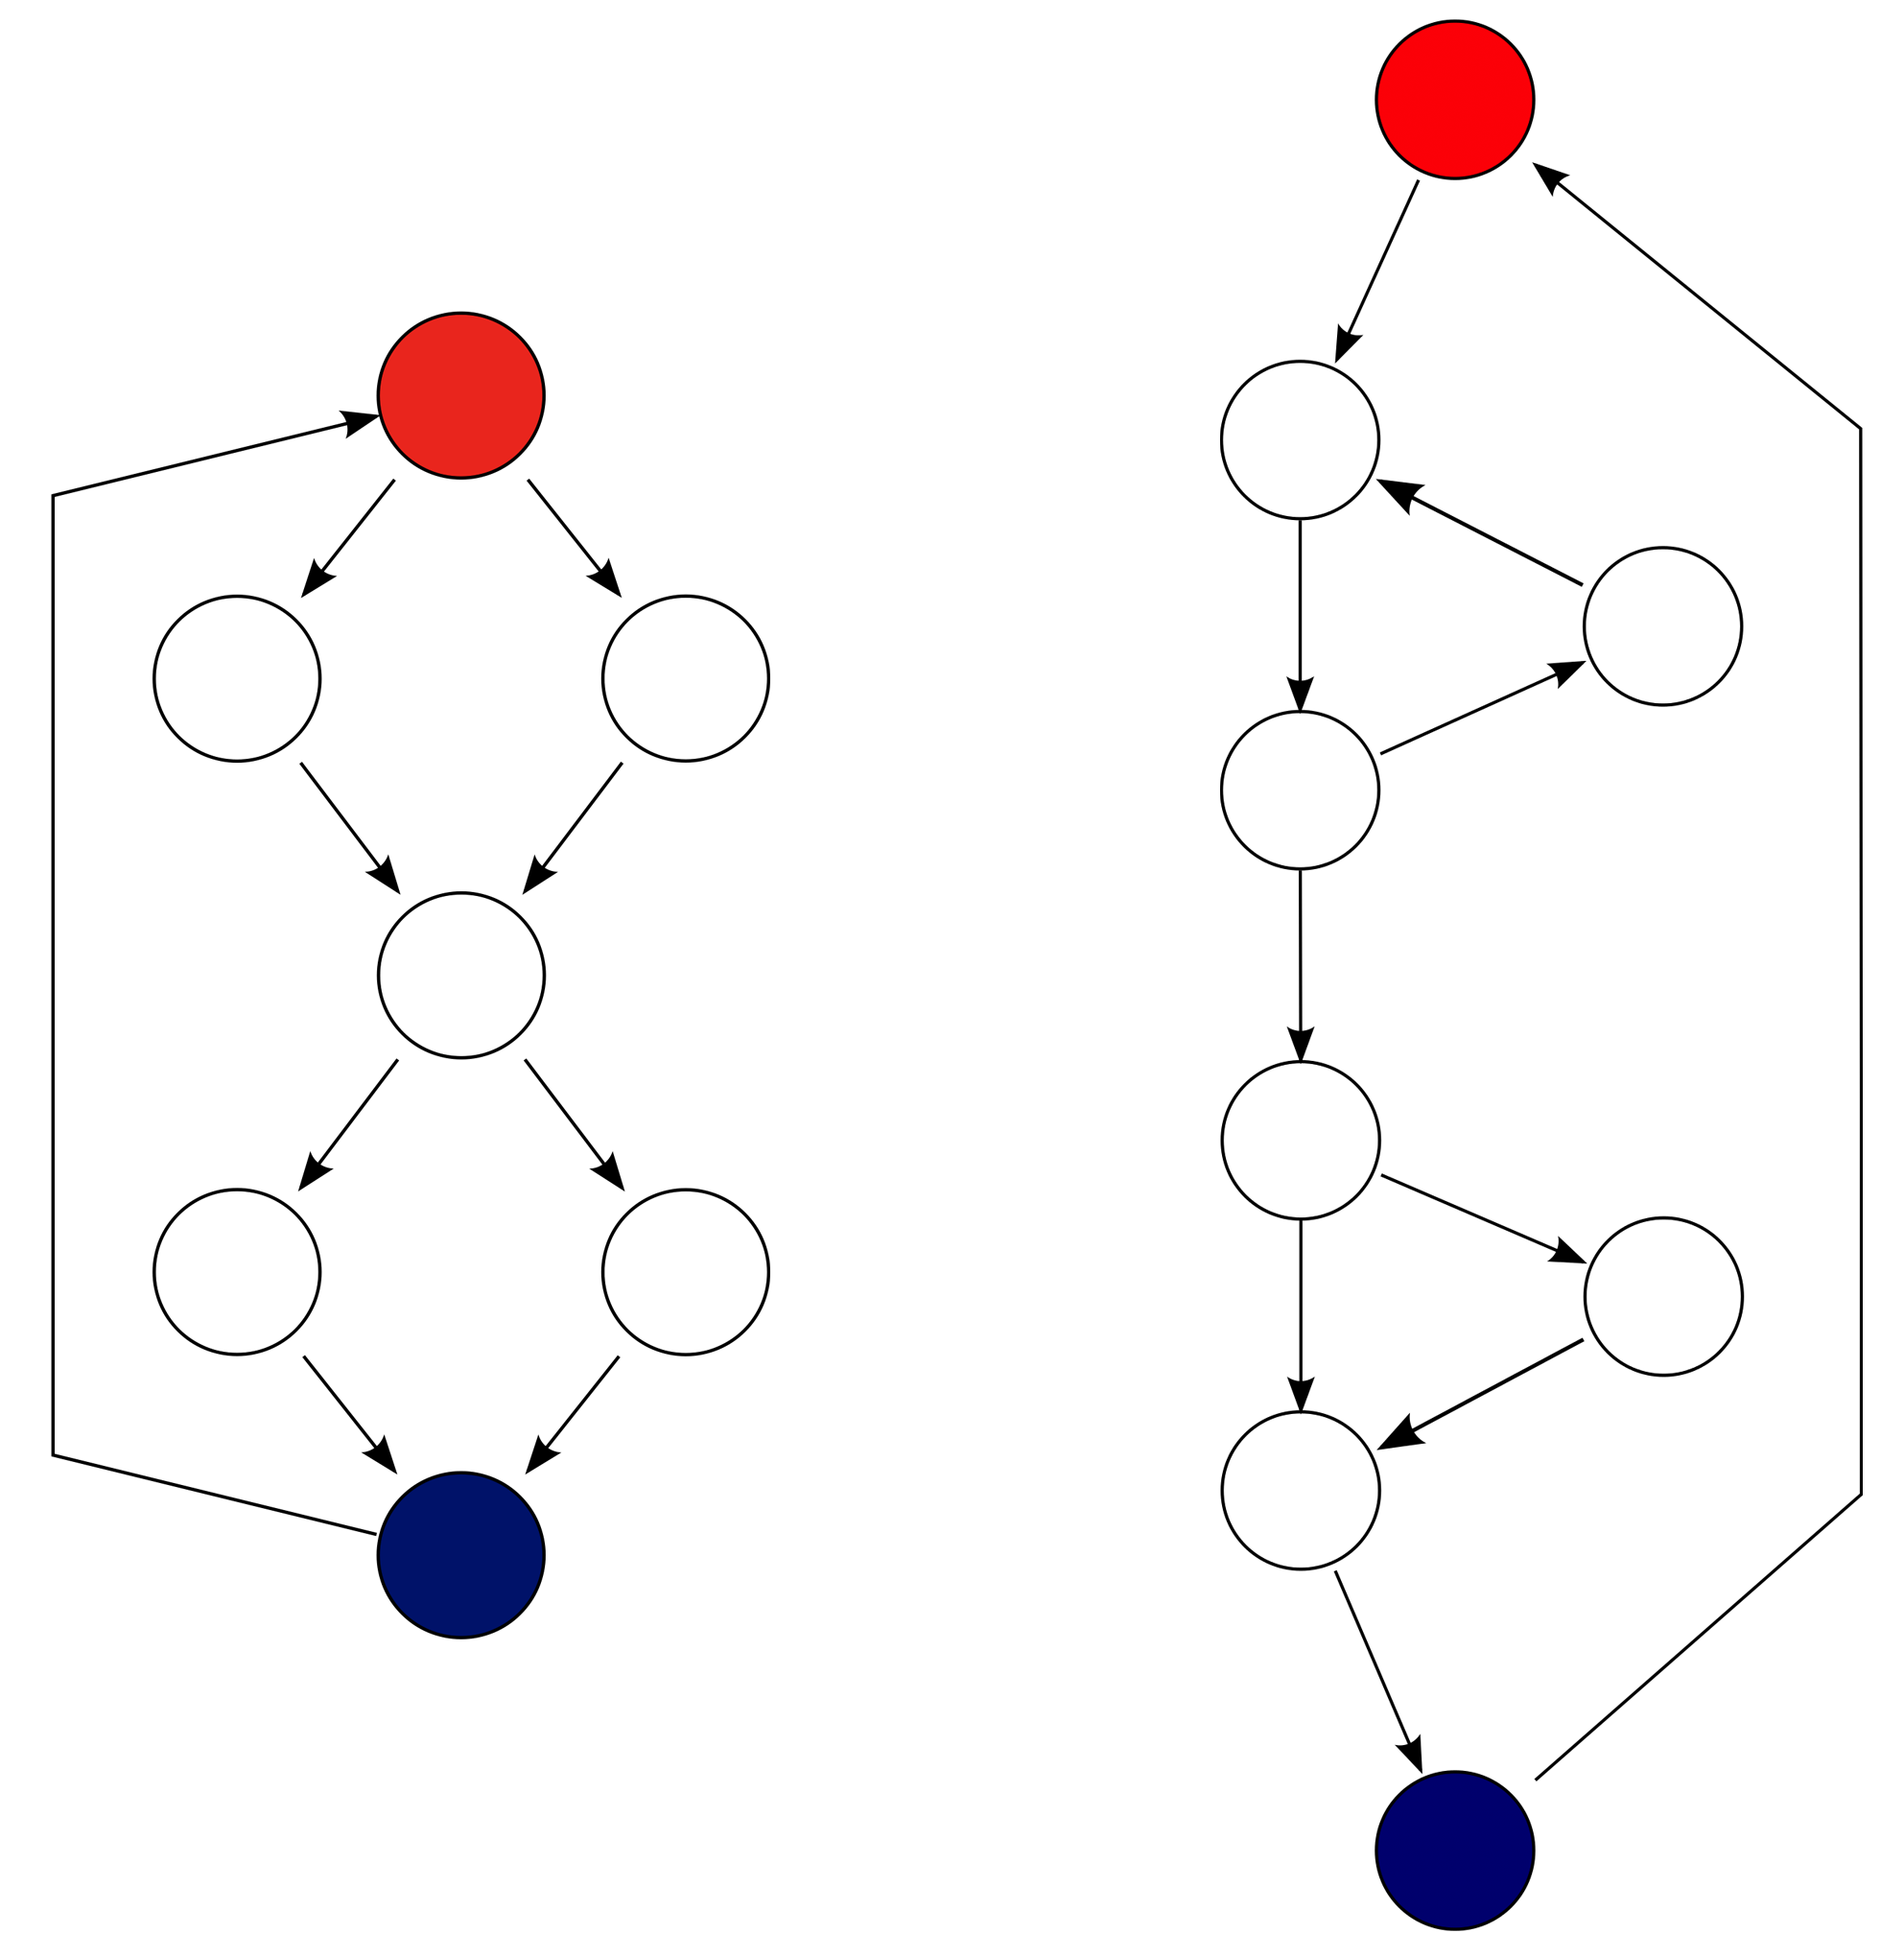
\includegraphics[width=0.6\textwidth]{cyclomatic}
	\caption{Examples of two simple cyclomatic graphs. Illustrations from Wikimedia, available under a public domain licence.}
	\label{fig:cyclomatic}
\end{figure}

%How, then, should one best apply it to gauge productivity?

Having said that, as \textcite{textbook} point out (p. 379), it is better for an appraisal system to be too simple than too complex.
Following that line of thought, Steria does not use cyclomatic complexity analysis to assess employees' productivity, as it is deemed too complicated.
One would instead prefer to spend more time and effort on appraising employees' accomplishments in areas that are harder to measure, such as for example cooperation, creativity, and initiative.

% (end)



\section{Further Discussion of Practice in Steria}
%In this section, I will discuss some software-specific approaches to qualitative appraisal.
%I will not discuss performance appraisal in general or common qualitative techniques such as the balanced scorecard method, 360-degree appraisal, and so on, since these methods are not unique to the software engineering field. 

As I have mentioned earlier, there is considerable difficulty associated with accurate, meaningful productivity measurement in this industry.
\textcite{textbook} emphasizes the need (p. 356) for supervisor appraisal to be based on objective performance records, which emphasizes the individual employee's responsibility for the organization's results in total and empowers employees to do their best.
Steria approaches this problem by letting qualitative assessment take the main role, while quantitative metrics are relegated to being a less important component in the appraisal system. 
The main forms of employee assessment used in Steria are supervisor, peer, and team appraisal. 
Though 360-degree appraisal is not explicitly instituted as the policy of choice, practice in Steria has significant similarities to this approach.
Furthermore, a behavioural checklist method \parencite[][371]{textbook} is the main method used for qualitative appraisal; appendix A includes an excerpt of Steria's competency framework. 

Another method used is peer evaluation within teams, both of general performance and quality of work.
\textcite{angel:howto} emphasizes the utility of continuous peer review:
\begin{quote}
	I have used technical reviews often because they reduce defects early, improve overall quality, and shorten the time to deliverable code. It also serves as a very good training tool. Using it to also measure productivity gives further value with little to no additional investment.
\end{quote}
On this point, practice in Steria is closely aligned with theory from the textbook, as peer appraisal is often associated with providing highly accurate and valid information \parencite[][357]{textbook}.
% http://www.examiner.com/article/article-9-how-to-measure-programmer-productivity




% TODO leave for last
\chapter{Conclusion}
% (fold)
Quantitative appraisal techniques used in the software business suffer from many of the limitations described by \textcite{textbook}, including criteria contamination, incentivizing short-term thinking, and not ignoring ``soft'' skills. 
Steria is aware of these shortcomings, and has chosen to use productivity measurement only to a limited extent and instead concentrate their resources on accurate, fair appraisal by qualitative means. 
I have outlined several common forms of quantitative productivity measurement, and while all of which are inadequate for being the sole means by which employees should be assessed, they all have strong points that make them suited for other forms of evaluation.


% (end)




\appendix

\chapter{Competency Framework Excerpt}
The next page is an excerpt of Steria's competency framework used for appraising employees' performance. 

Please note that this document is \textbf{CONFIDENTIAL} and is not intended for further dissemination. 

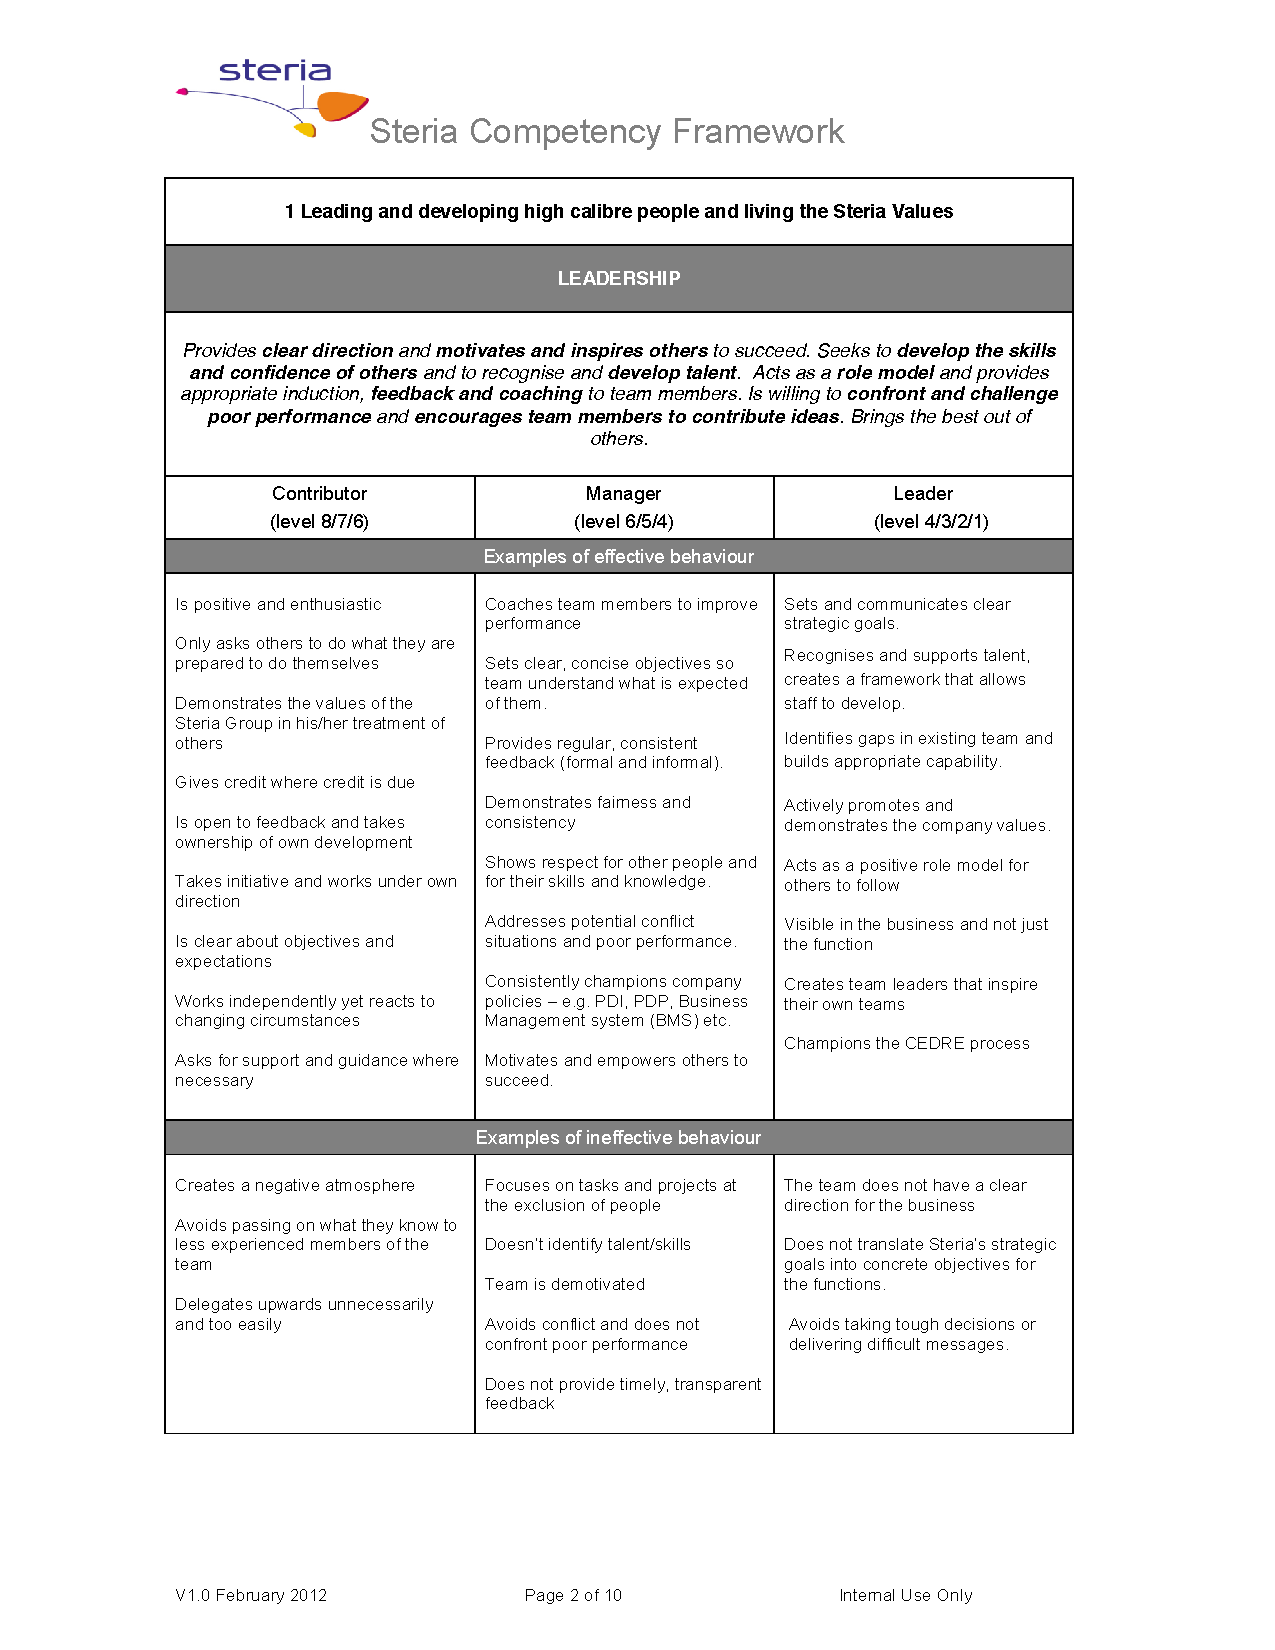
\includepdf{framework}


% TODO still alle spørsmål!
\chapter{Interview Questions}
% (fold)
These questions concern both this report and my group project on compensation. Correspondence took place by e-mail.
\begin{enumerate}[leftmargin=*]
	\item Do you use salary grades or a sliding scale?
	\item Do you primarily use hourly wages, salaries, or a combination of the two?
	\item To what extent is performance-based compensation used?
	\item How often are salaries reevaluated?
	\item What is the overtime policy? Is use of overtime common, and under what circumstances?
	\item Is compensation considered a private matter or is it discussed freely?
	\item Do you have a compensation policy such as being market leading or competitive?
	\item Do you have ``escalator clauses'', i.e., contract clauses that tie a certain part of the salary to increases in cost of living in general?
	\item Is collective or individual bargaining more common? Why?
	\item How is good day-to-day performance rewarded and recognized?
	\item How do you attract new employees, and what do you do to retain old ones?
	\item How is the need for hiring evaluated?
	\item What kinds of non-monetary compensation do you offer?
	\item How are employees' performance evaluated?
	\item Are employees appraised by anyone apart from their supervisors, e.g., team members?
	\item Is any form of automated assessment used, such as counting lines of code written or the like? How, in that case, is it used?
\end{enumerate}

% (end)




\chapter{Letter of Thanks}
The next page is a copy of the letter I sent to Mrs. Skilbrigt to express my gratitude. 
In the interest of truthfulness, I provided the letter as it was sent, in its original Norwegian.

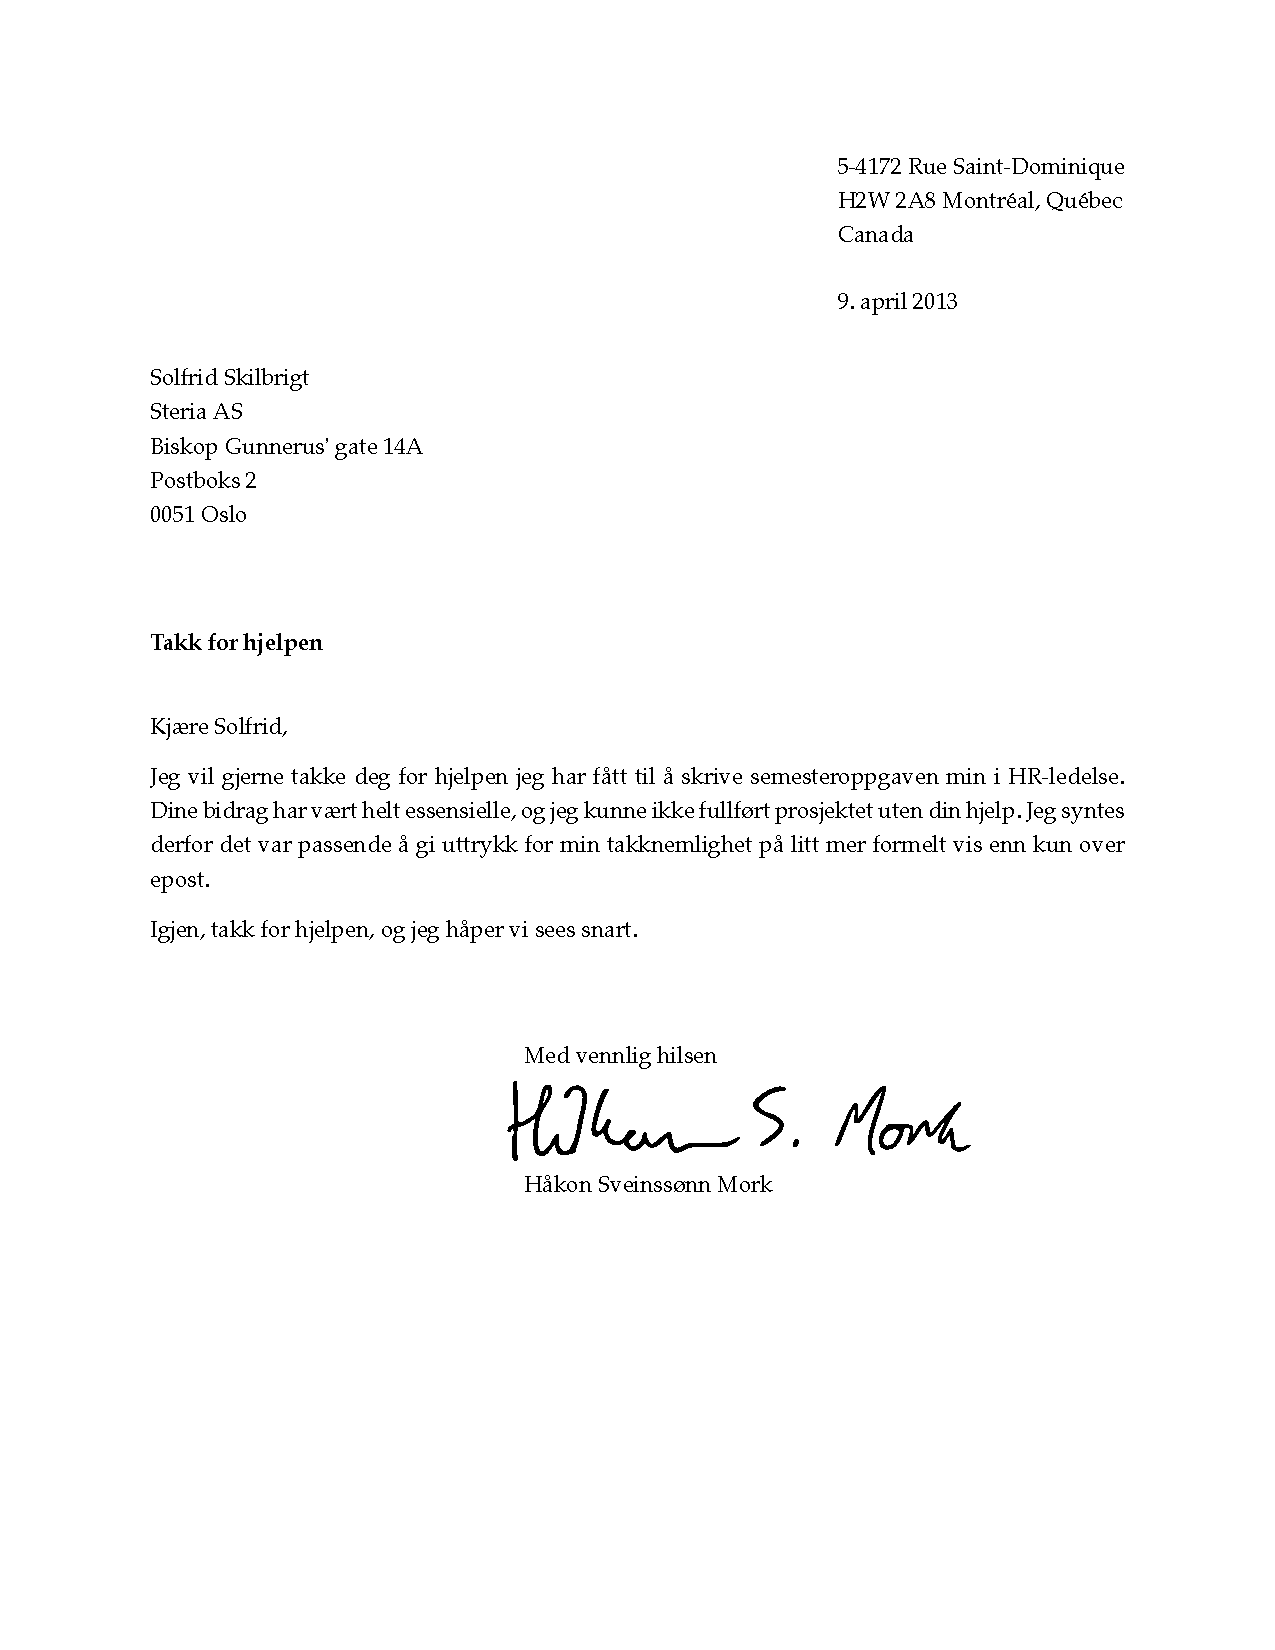
\includepdf{../takkebrev/takkebrev-include.pdf}


\chapter{Business Card}

\includegraphics[width=\textwidth]{visittkort}


%\nocite{*}
\printbibliography
\phantomsection
\addcontentsline{toc}{chapter}{Bibliography}

\end{document}


%http://www.sei.cmu.edu/library/abstracts/reports/92tr020.cfm
%http://scholar.google.co.uk/scholar?q=lines+of+code&btnG=&hl=en&as_sdt=0%2C5
